% WR figure exported by sim_ui.py -- 2026-09-19 11:35:12
%
% Preamble (once, in your thesis):
%   \usepackage{pgfplots}
%   \pgfplotsset{compat=1.18}
%
% Use:
%   \begin{figure}[htbp]\centering
%     \input{wr_convergence}
%     \caption{...}\label{fig:...}
%   \end{figure}
%
% \input nests (unlike \include), so this works inside a chapter file the root
% already \includes. Pasting the body below inline works too -- the \definecolor
% lines may then be hoisted into the preamble and dropped from each figure.
%
% Series are thinned to ~2000 points each (min/max decimation, so spikes are
% preserved); edit _PGF_MAX_PTS in sim_ui.py for the full-resolution data.
%
% Run: coupling_mode=voltage-driven; precondition=on (optimized); interface_form=Thevenin (V source); use_t_floor=bare dt; interface_consistency=accumulated; N_field_windows=100; N_xyce_samples=200; xyce_integration_method=Backward-Euler (maxord=1)

\definecolor{C0}{HTML}{1F77B4}
\definecolor{C1}{HTML}{FF7F0E}
\definecolor{C2}{HTML}{2CA02C}
\definecolor{C3}{HTML}{D62728}

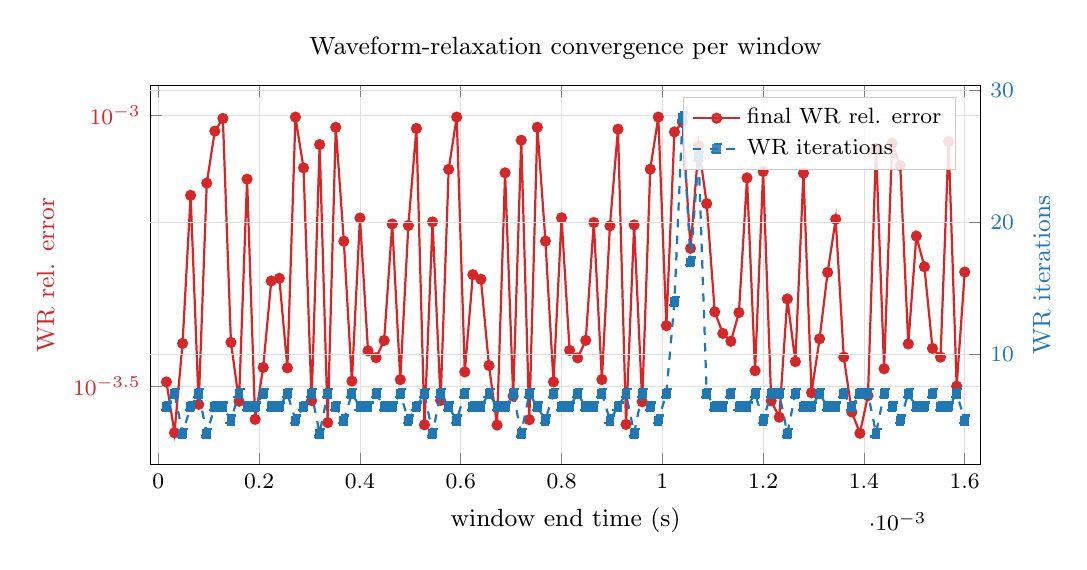
\begin{tikzpicture}
\begin{axis}[
  width=\linewidth,
  height=6.4cm,
  title={Waveform-relaxation convergence per window},
  xlabel={window end time (s)},
  ylabel={WR rel. error},
  grid=both,
  grid style={line width=.2pt, draw=gray!25},
  legend pos=north east,
  legend cell align=left,
  legend style={font=\footnotesize, fill=white, fill opacity=0.85, text opacity=1, draw=gray!40},
  tick label style={font=\footnotesize},
  label style={font=\small},
  title style={font=\small},
  scaled x ticks=true,
  xmin=-1.568e-05,
  xmax=0.00163168,
  ymode=log,
  axis y line*=left,
  ylabel style={color=C3},
  yticklabel style={color=C3}
]
  \addplot[color=C3, line width=0.8pt, mark=*, mark size=1.6pt] coordinates {
    (1.6e-05,0.0003217) (3.2e-05,0.0002592) (4.8e-05,0.000379) (6.4e-05,0.0007112) (8e-05,0.0002925) (9.6e-05,0.0007493)
    (0.000112,0.0009342) (0.000128,0.0009857) (0.000144,0.0003806) (0.00016,0.0002963) (0.000176,0.0007619) (0.000192,0.0002744)
    (0.000208,0.0003422) (0.000224,0.0004941) (0.00024,0.0004997) (0.000256,0.0003416) (0.000272,0.0009917) (0.000288,0.0007994)
    (0.000304,0.0002973) (0.00032,0.0008824) (0.000336,0.0002706) (0.000352,0.0009494) (0.000368,0.000585) (0.000384,0.0003229)
    (0.0004,0.0006458) (0.000416,0.0003672) (0.000432,0.0003567) (0.000448,0.0003837) (0.000464,0.0006296) (0.00048,0.0003249)
    (0.000496,0.0006256) (0.000512,0.0009448) (0.000528,0.0002681) (0.000544,0.0006351) (0.00056,0.0002975) (0.000576,0.0007943)
    (0.000592,0.0009918) (0.000608,0.0003357) (0.000624,0.0005076) (0.00064,0.0004978) (0.000656,0.000345) (0.000672,0.0002678)
    (0.000688,0.0007826) (0.000704,0.0003028) (0.00072,0.0008988) (0.000736,0.000274) (0.000752,0.0009497) (0.000768,0.0005854)
    (0.000784,0.0003218) (0.0008,0.0006464) (0.000816,0.0003679) (0.000832,0.0003564) (0.000848,0.000384) (0.000864,0.0006336)
    (0.00088,0.000325) (0.000896,0.0006247) (0.000912,0.0009421) (0.000928,0.0002686) (0.000944,0.0006271) (0.00096,0.0002958)
    (0.000976,0.000795) (0.000992,0.0009917) (0.001008,0.0004086) (0.001024,0.0009311) (0.00104,0.0009701) (0.001056,0.0005677)
    (0.001072,0.0008779) (0.001088,0.0006864) (0.001104,0.0004334) (0.00112,0.0003954) (0.001136,0.0003824) (0.001152,0.0004321)
    (0.001168,0.000766) (0.001184,0.0003375) (0.0012,0.0007872) (0.001216,0.0002968) (0.001232,0.0002769) (0.001248,0.0004578)
    (0.001264,0.0003507) (0.00128,0.0007816) (0.001296,0.0003073) (0.001312,0.0003865) (0.001328,0.0005126) (0.001344,0.0006423)
    (0.00136,0.0003576) (0.001376,0.0002831) (0.001392,0.0002587) (0.001408,0.0003035) (0.001424,0.0008692) (0.00144,0.0003403)
    (0.001456,0.0008871) (0.001472,0.0008072) (0.001488,0.0003782) (0.001504,0.000598) (0.00152,0.0005249) (0.001536,0.0003711)
    (0.001552,0.0003575) (0.001568,0.0008941) (0.001584,0.000316) (0.0016,0.0005133)
  };
\end{axis}
\begin{axis}[
  width=\linewidth,
  height=6.4cm,
  title={},
  xlabel={},
  ylabel={WR iterations},
  grid=both,
  grid style={line width=.2pt, draw=gray!25},
  legend pos=north east,
  legend cell align=left,
  legend style={font=\footnotesize, fill=white, fill opacity=0.85, text opacity=1, draw=gray!40},
  tick label style={font=\footnotesize},
  label style={font=\small},
  title style={font=\small},
  scaled x ticks=true,
  xmin=-1.568e-05,
  xmax=0.00163168,
  axis y line*=right,
  axis x line=none,
  ylabel style={color=C0},
  yticklabel style={color=C0}
]
  \addlegendimage{color=C3, line width=0.8pt, mark=*, mark size=1.6pt}
  \addlegendentry{final WR rel. error}
  \addplot[color=C0, line width=0.8pt, dashed, mark=square*, mark size=1.6pt] coordinates {
    (1.6e-05,6) (3.2e-05,7) (4.8e-05,4) (6.4e-05,6) (8e-05,7) (9.6e-05,4)
    (0.000112,6) (0.000128,6) (0.000144,5) (0.00016,7) (0.000176,6) (0.000192,6)
    (0.000208,7) (0.000224,6) (0.00024,6) (0.000256,7) (0.000272,5) (0.000288,6)
    (0.000304,7) (0.00032,4) (0.000336,7) (0.000352,6) (0.000368,5) (0.000384,7)
    (0.0004,6) (0.000416,6) (0.000432,7) (0.000448,6) (0.000464,6) (0.00048,7)
    (0.000496,5) (0.000512,6) (0.000528,7) (0.000544,4) (0.00056,7) (0.000576,6)
    (0.000592,5) (0.000608,7) (0.000624,6) (0.00064,6) (0.000656,7) (0.000672,6)
    (0.000688,6) (0.000704,7) (0.00072,4) (0.000736,7) (0.000752,6) (0.000768,5)
    (0.000784,7) (0.0008,6) (0.000816,6) (0.000832,7) (0.000848,6) (0.000864,6)
    (0.00088,7) (0.000896,5) (0.000912,6) (0.000928,7) (0.000944,4) (0.00096,7)
    (0.000976,6) (0.000992,5) (0.001008,7) (0.001024,14) (0.00104,28) (0.001056,17)
    (0.001072,25) (0.001088,7) (0.001104,6) (0.00112,6) (0.001136,7) (0.001152,6)
    (0.001168,6) (0.001184,7) (0.0012,5) (0.001216,7) (0.001232,7) (0.001248,4)
    (0.001264,7) (0.00128,6) (0.001296,6) (0.001312,7) (0.001328,6) (0.001344,6)
    (0.00136,7) (0.001376,6) (0.001392,7) (0.001408,7) (0.001424,4) (0.00144,7)
    (0.001456,6) (0.001472,5) (0.001488,7) (0.001504,6) (0.00152,6) (0.001536,7)
    (0.001552,6) (0.001568,6) (0.001584,7) (0.0016,5)
  };
  \addlegendentry{WR iterations}
\end{axis}
\end{tikzpicture}
